\chapter{تجهيز ملف المنشأة في السجل الصناعي}
\label{ch:03-register}
\section{ما ملف المنشأة؟}
\label{sec:register-file}

لكل منشأة ملف واحد في تطبيق «السجل الصناعي». يجمع هذا الملف كل ما نعرفه عنها: من هي، وأين تقع، ومن يملكها، وماذا تنتج. وتعتمد عليه الخطة لتختار المنشآت، ويعتمد عليه النموذج ليملأ بعض الإجابات مسبقاً.

\begin{table}[H]
\centering
\caption{بيانات الملف وبيانات الجولة}
\label{tab:register-file}
\begin{tabularx}{\linewidth}{Y Y}
\rcHeaderRow
\thh{ملف المنشأة} & \thh{بيانات الجولة}\\
يبقى مع المنشأة ويتحدّث عند الحاجة. & تخص فترة مسح واحدة، مثل جولة 2026.\\
الاسم والموقع والمالك والقيد والمنتجات والآلات. & الإجابات التي جُمعت عن تلك الفترة.\\
يعدّله موظف السجل. & يجمعها الباحث وتُعتمد في مسار المراجعة.\\
\end{tabularx}
\end{table}

\textbf{افتح الملف:} من تطبيق «السجل الصناعي» افتح «المنشآت الصناعية»، ثم اضغط اسم المنشأة. تُفتح صفحتها على تبويب «نظرة عامة».

\begin{figure}[H]
\centering
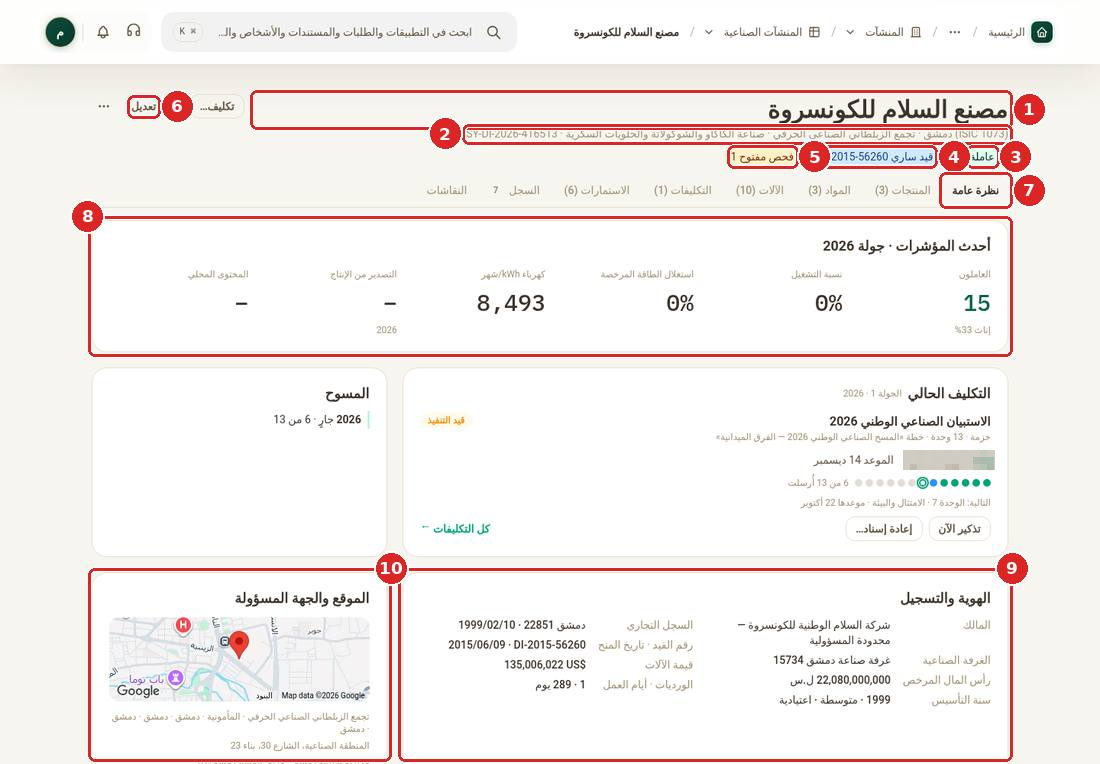
\includegraphics[width=\linewidth]{assets/screens/register-facility-top-ar.png}
\caption{أعلى صفحة المنشأة}
\label{fig:register-facility-top}
\shotnote{هذه صفحة ملف منشأة صناعية، وفيها أهم ما يلزم قبل المسح وبعده. تفيدك في التأكد من هوية المنشأة وحالتها قبل أن تُسند إليها أي عمل. ابدأ دائماً من الاسم والحالة، ثم انتقل إلى التبويبات للتفاصيل. ① اسم المنشأة. ② الرقم الوطني والمحافظة والنشاط. ③ حالة التشغيل: هنا «عاملة». ④ القيد الساري في السجل الصناعي. ⑤ «فحص مفتوح»: نتيجة فحص جودة تحتاج متابعة. ⑥ «تعديل». ⑦ تبويبات الملف. ⑧ «أحدث المؤشرات»: أرقام آخر جولة معتمدة. ⑨ «الهوية والتسجيل». ⑩ «الموقع والجهة المسؤولة».}
\end{figure}

\begin{rcnote}[تطبيق المثال: ملف مصنع الأفق]
يحمل ملف المثال هذه البيانات: الاسم «مصنع الأفق للصناعات الغذائية»، والمحافظة ريف دمشق، والنشاط صناعة المنتجات الغذائية، وحالة التشغيل «عاملة». أما «24 عاملاً و3 أيام توقف في أيلول 2026» فليست من الملف؛ إنها بيانات جولة سيجمعها عمر في الفصل السادس.
\end{rcnote}

\section{ما السجلات المرتبطة بالمنشأة؟}
\label{sec:register-linked}

لا يحفظ الملف كل شيء في صفحة واحدة. فبعض البيانات سجلات مستقلة مرتبطة بالمنشأة، ولكل منها صفحته. وكل اسم أو رمز أخضر في الصفحة رابط يفتح صفحة ذلك السجل.

\begin{table}[H]
\centering
\caption{السجلات المرتبطة بالمنشأة}
\label{tab:register-linked}
\begin{tabularx}{\linewidth}{R{3cm} Y}
\rcHeaderRow
\thh{السجل} & \thh{ماذا يحفظ؟}\\
المالك & الكيان القانوني الذي يملك المنشأة، وكل منشآته الأخرى.\\
قيد السجل الصناعي & رقم القيد ورأس المال وقيمة الآلات والورديات.\\
المنتجات & كل منتج، مع رمز HS والطاقة المرخصة سنوياً.\\
المواد الأولية & المادة ومصدرها واستهلاكها الشهري.\\
الآلات & عدد الآلات ومتوسط عمرها ومستوى أتمتتها.\\
نشاط ISIC & النشاط الصناعي للمنشأة وفق التصنيف الدولي.\\
\end{tabularx}
\end{table}

\begin{figure}[H]
\centering
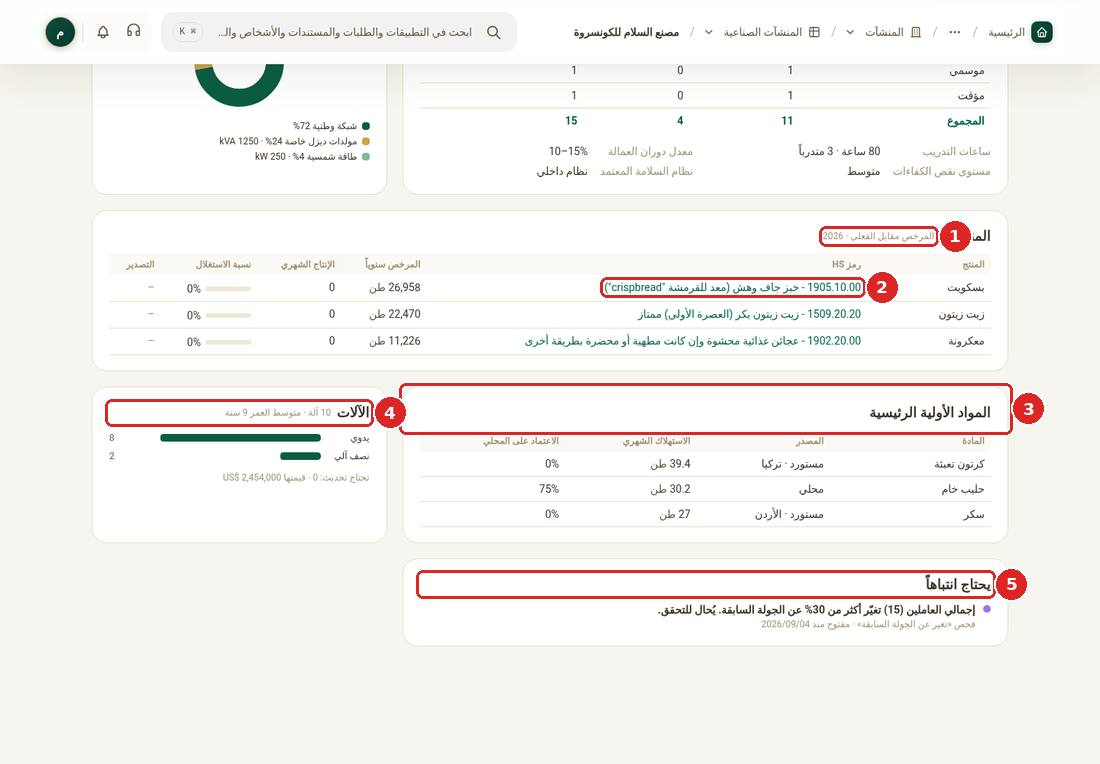
\includegraphics[width=\linewidth]{assets/screens/register-facility-assets-ar.jpg}
\caption{المنتجات والمواد والآلات في صفحة المنشأة}
\label{fig:register-facility-assets}
\shotnote{يعرض أسفل صفحة المنشأة السجلات المرتبطة بها في جداول قصيرة. تفيدك في معرفة ما تملكه المنشأة وتنتجه قبل المسح؛ فهذه البيانات تظهر لاحقاً مملوءة مسبقاً في النموذج. ① «المرخص مقابل الفعلي»: مقارنة الطاقة المرخصة بالإنتاج. ② رمز HS: رابط إلى صفحة الرمز. ③ «المواد الأولية الرئيسية». ④ «الآلات». ⑤ «يحتاج انتباهاً»: نتيجة فحص جودة على المنشأة.}
\end{figure}

\begin{rcnote}[تطبيق المثال]
مالك مصنع الأفق هو «شركة الأفق للأغذية». وللمصنع قيد ساري، ومنتجان: «معلبات الخضار» و«عصير الفواكه». ستظهر هذه البيانات لعمر مملوءة مسبقاً عندما يفتح النموذج، فيكتفي بالتحقق منها.
\end{rcnote}

\section{حالتا المنشأة: التشغيل والتسجيل}
\label{sec:register-status}

لكل منشأة حالتان مختلفتان، فلا تخلط بينهما:

\begin{itemize}
\item \textbf{حالة التشغيل:} هل المنشأة تعمل؟ مثل «عاملة» أو «متوقفة»، أو مغلقة نهائياً. تستبعد خطة المسح المنشآت المغلقة.
\item \textbf{حالة التسجيل:} هل تحقق السجل من المنشأة؟ لها ثلاث قيم: «مسجلة»، و«مكتشفة ميدانياً»، و«قيد التحقق».
\end{itemize}

كل منشأة غير مسجلة تحمل شارة بحالتها في صفحتها، حتى يتحقق منها موظف السجل ويغيّرها إلى «مسجلة».

\begin{rcnote}[تطبيق المثال]
مصنع الأفق «عاملة» و«مسجلة»، فتشمله الخطة. ولو أُغلق المصنع لاستبعدته الخطة، ولن يصل تكليفه إلى عمر حتى لو كان كل شيء آخر صحيحاً.
\end{rcnote}

\section{اربط المنشأة بفريق المسح}
\label{sec:register-team}

عرفنا في الفصل~\ref{ch:02-roles} أن الخطة تقرأ حقل «فريق المسح» في ملف المنشأة لتختار الباحث. لذلك يجب أن يحمل الملف الفريق الصحيح قبل إطلاق الخطة.

\begin{enumerate}
\item افتح ملف المنشأة، ثم اضغط «تعديل».
\item اختر الفريق في حقل «فريق المسح».
\item احفظ، ثم تأكد أن اسم الفريق ظهر في الملف.
\end{enumerate}

\begin{rcnote}[تطبيق المثال]
يفتح يوسف ملف مصنع الأفق، ويختار «فريق مسح الأفق» في حقل «فريق المسح»، ثم يحفظ. بهذا تجد الخطة عمر داخل الفريق. وإذا ترك يوسف الحقل فارغاً، فلن تجد الخطة مرشحاً للمصنع.
\end{rcnote}

\section{أضف منشأة جديدة}
\label{sec:register-new}

قد تحتاج إلى منشأة غير موجودة في السجل. لذلك طريقتان:

\begin{enumerate}
\item \textbf{إضافة سريعة:} من «المنشآت الصناعية» اضغط «إضافة» واكتب اسم المنشأة فقط. تأخذ حالة التسجيل «مكتشفة ميدانياً» تلقائياً. بعدها يمكن تكليفها من القائمة: «تكليف بنموذج» ثم «ضمن خطة».
\item \textbf{اكتشاف ميداني:} إذا صادف الباحث منشأة غير مسجلة، يبدأ لها النموذج الأول باستخدام «طلب جديد»، ثم يختار «غير موجودة في القائمة» في منتقي المنشأة. عند الاعتماد الأخير تُنشأ المنشأة في السجل بحالة «مكتشفة ميدانياً».
\end{enumerate}

في الحالتين، يكمل موظف السجل بيانات المنشأة الجديدة، ثم يغيّر حالة تسجيلها إلى «قيد التحقق» ثم «مسجلة».

\begin{figure}[H]
\centering
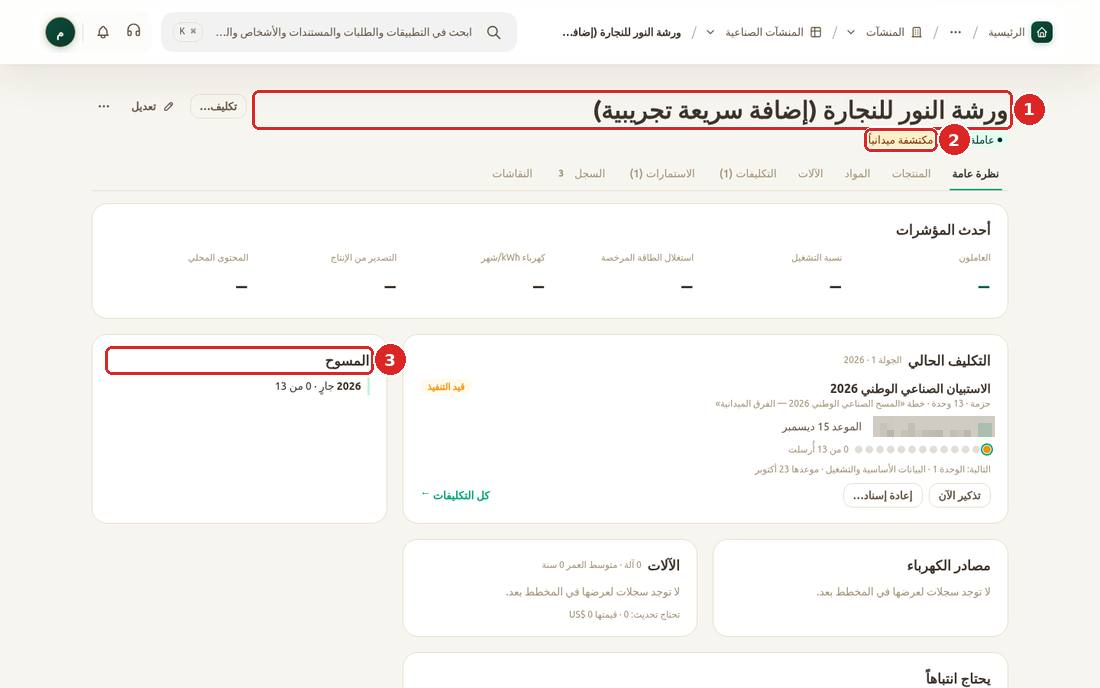
\includegraphics[width=\linewidth]{assets/screens/register-quick-add-ar.png}
\caption{منشأة أُضيفت بالاسم فقط}
\label{fig:register-quick-add}
\shotnote{تعرض الصورة منشأة أُضيفت بالإضافة السريعة، فلا يحتوي ملفها إلا على الاسم. تفيدك في التعرف على المنشأة الجديدة من شارتها، ومعرفة أن ملفها يحتاج إلى استكمال. ① الاسم: البيان الوحيد المطلوب عند الإضافة. ② «مكتشفة ميدانياً»: حالة التسجيل الافتراضية. ③ «المسوح»: «0 من 13» بعد إضافتها إلى الخطة.}
\end{figure}

\begin{rcnote}[تطبيق المثال]
أثناء زيارة عمر لريف دمشق، يجد مخبزاً صغيراً بجوار مصنع الأفق غير مسجل. يبدأ له نموذجاً جديداً ويختار «غير موجودة في القائمة». بعد الاعتماد يظهر المخبز في السجل بحالة «مكتشفة ميدانياً»، فيكمل يوسف ملفه ويغيّر حالته إلى «مسجلة».
\end{rcnote}

\section{كيف تصل بيانات المسح إلى الملف؟}
\label{sec:register-flow}

يتبادل الملف والنموذج البيانات في الاتجاهين:

\begin{enumerate}
\item \textbf{من الملف إلى النموذج:} تأتي بعض الإجابات مملوءة مسبقاً، وعليها شارة «من السجل». يتحقق منها الباحث ويعدّل ما تغيّر.
\item \textbf{التعديل قابل للتراجع:} إذا عدّل الباحث قيمة، يظهر بجانبها «كانت …» وزر «استعادة».
\item \textbf{سجل الجولة يسبق الإجابات:} يُنشأ «سجل الجولة» الخاص بالفترة عند تكليف المنشأة بالحزمة، قبل أن تبدأ التعبئة.
\item \textbf{من النموذج إلى الملف:} بعد الاعتماد الأخير فقط، تُكتب الإجابات في ملف المنشأة وفي سجل الجولة.
\item \textbf{سجل جولة واحد:} لكل منشأة سجل جولة واحد في كل جولة. ولا يُنشأ سجل ثانٍ للجولة نفسها.
\end{enumerate}

\begin{rcnote}[تطبيق المثال]
يفتح عمر النموذج فيجد اسم مصنع الأفق ونشاطه مملوءين «من السجل». يُنشأ سجل جولة أيلول 2026 للمصنع عندما تطلق سارة الخطة. وبعد أن توقّع رنا على الإجابة، يظهر عدد العاملين 24 في «أحدث المؤشرات» بصفحة الملف.
\end{rcnote}

\begin{rcchecklist}[قبل إطلاق المسح على مصنع الأفق]
\begin{checklist}
\item ملف المصنع موجود، واسمه ومحافظته ونشاطه صحيحة.
\item المصنع غير مغلق، وحالة تسجيله معروفة.
\item حقل «فريق المسح» يحمل «فريق مسح الأفق».
\item المالك والقيد والمنتجات مرتبطة بالملف.
\item أعرف أن بيانات الجولة لا تدخل الملف إلا بعد الاعتماد الأخير.
\end{checklist}
\end{rcchecklist}

بعد تجهيز الملف، نبني في الفصل~\ref{ch:04-forms} نموذج «بيانات التشغيل» الذي سيجمع عمر به بيانات المصنع.
